\chapter{Plataforma Abierta de Teleoperación}
\begin{flushright}
\begin{minipage}{0,7\textwidth}
En este cap\'itulo se presenta el diseño de una arquitectura de control en tiempo real para una plataforma abierta de teleoperación compuesta por un brazo robótico de tipo antropomórfico. Este robot es actúa a través de dispositivos hidráulicos, operando en un entorno remoto y realimentando a un dispositivo maestro cinemáticamente idéntico, cerrando los bucles de control en fuerza. Son analizados los requerimientos de control para dispositivos hápticos. Se propone una arquitectura hardware/software. La arquitectura software propuesta se basa en técnicas de computación distribuida, la información acerca de ambos manipuladores se comparte por medio de una red local de internet.
\end{minipage}
\end{flushright}




\newpage
\section{Arquitectura General}

Como se muestra en la figura \ref{fig:arquitectura} el sistema robótico de teleoperación que se utilizar\'a en este trabajo se compone de las siguientes partes:\\

\begin{itemize}
\item Un manipulador hidráulico de seis grados de libertad (GDL) de la firma Kraft Telerobotics\textregistered
\item Un Efector final de tipo pinza
\item Dos controladores de tiempo real NI PXIe-1078
\item Un dispositivo maestro de seis grados de libertad
\end{itemize}

La arquitectura de control ha sido diseñada para compartir toda la información entre los sistemas maestro y el esclavo a través de Internet. En esta plataforma de teleoperación la información entre el maestro y el esclavo es compartida a través de una red local(LAN).\\


\begin{figure}[hbt!]
\caption{Arquitectura de la Plataforma de Teleoperacion}
\label{fig:arquitectura}
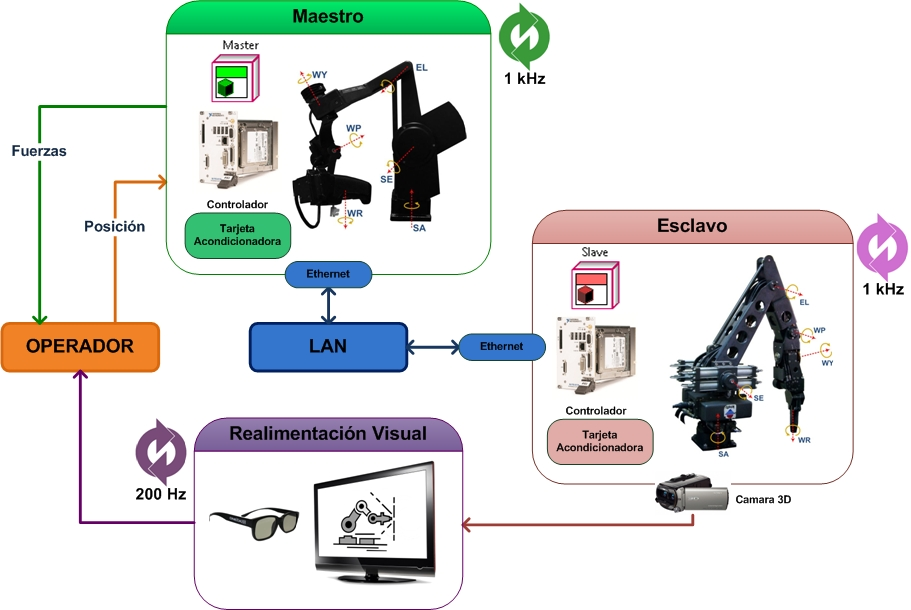
\includegraphics[scale=0.7]{FiguresP/ManufacturerArquitecture}
\end{figure}




El controlador de tiempo real del sistema maestro recibe mediciones de la posición y de la presión en los actuadores hidráulicos y la envía al controlador de tiempo real del dispositivo maestro que la procesa. El dispositivo maestro brinda una reflexión  de fuerzas al usuario basado en la información del esclavo, lee la posición actual de las articulaciones y calcula la posición y orientación del manipulador esclavo deseadas. El  dispositivo esclavo  usa esta información para  cerrar los bucles control (PI) de posición en cada articulación.\\

El protocolo de red utilizado para este sistema de teleoperación fue UDP (User Datagram Protocol). El protocolo UDP usa  un modelo de transmisión simple con un mecanismo mínimo\cite{zhao2006contrast} .

%Una de las ventajas del protocolo UDP
%La frecuencia ideal para los sistemas de teleoperación con reales de 1 KHz 


\section{Requerimientos del Sistema de Control}

En esta sección se describen las especificaciones de los componentes de la arquitectura de control para un sistema de teleoperación tipo maestro-esclavo 6 GDL. El sistema desarrollado debe contar con realimentación háptica  en los primeros tres  GDL, así como una realimentación visual y auditiva. La realimentación brindada al usuario es resultado de la interacción física con el entorno remoto.\\

Para lograr una transición suave en las gráficas o una realimentación visual aceptable es necesaria al menos una frecuencia de actualización de imágenes de al menos 50 Hz. en caso de requerirse una visión estereoscópica la frecuencia deberá aumentar por lo menos a 100 Hz. Uno de los requisitos de un sistema de teleoperaci\'on h\'aptico es que la frecuencia de realimentaci\'on visual sea suficiente para que el usuario tenga una experiencia similar a la que tendr\'ia si lo estuviera manipulando directamente. Es decir el usuario experimenta de forma coherente la información de forma visual y táctil. As\'i mismo la realimentación de fuerza también  requiere de una alta velocidad de actualización no solo para proporcionar una sensación realista sino también para asegurar la estabilidad. Se considera que es necesaria una frecuencia de actualización en tiempo real de al menos 1 KHz para alcanzar una sensación h\'aptica aceptable. Por otra parte los retardos en la transmisión de fuerzas pueden producir inestabilidades en el sistema h\'aptico al no ser consideradas en la fase de diseño.\\


 para sistemas de teleoperación sin realimentación háptica, las velocidades de actualización en tiempo real no son necesarias, debido a que la información visual es realimentada al usuario de forma unidireccional, dado que no afecta el comportamiento de los controladores del robot. 


El realismo de la interacción es denominado \textsc{transparencia}. La transparencia del sistema teleoperado es determinada por el algoritmo de control bilateral. Un requisito fundamental de un sistema de telemanipulaci\'on funcional es garantizar la estabilidad del sistema para todas las circunstancias que puedan ser encontradas durante la operación.\\


Para satisfacer estos requerimientos, se propone una arquitectura de red que procese las señales y realice los cálculos necesarios para el control del sistema en tiempo real. Esta arquitectura de control permite la conexión simult\'anea de los sistemas a través de Internet, lo cual es ideal para permitir una arquitectura abierta que permita a los desarrolladores programar y probar  sus aplicaciones  o estrategias de control.


%The realism of this reflected interaction is called the transparency of the system [1]. The obtainable transparency is amongst others
%determined by the implemented bilateral control algorithm. A fundamental requirement for a useful telemanipulation system is that it is guaranteed to be stable given all possible circumstances that can be encountered during operation.


\newpage
\section{Descripción detallada de la plataforma de teleoperaci\'on}

A continuación se describen algunos aspectos fundamentales a cerca de la plataforma experimental de teleoperación en la cual está basado el presente trabajo \cite{Galiana2012}. La intenci\'on es mejorar algunos aspectos físicos de la misma con la finalidad de conseguir un mejor rendimiento en cuanto a percepción del operador y con ello conseguir un menor tiempo en la ejecución de distintas tareas aplicando distintos algoritmos de control bilateral.\\

Se ha partido de dispositivos existentes en el grupo de investigación, dado que la realización de una plataforma de teleoperación supone un elevado coste y una gran inversión de tiempo. Se propone que sea totalmente abierta, con el propósito de que no solamente permita comprobar experimentalmente los algoritmos presentados, sino que adem\'as permita realizar cualquier otro tipo de pruebas, experimentos o investigaciones en el área de teleoperación.\\

Los movimientos ejercidos en el brazo maestro son reproducidos en el robot esclavo. Se caracteriza porque utiliza la arquitectura de control Fuerza - Posición, con lo cual el sistema mediante el maestro refleja fuerzas (alrededor del 10\%) al operador para que pueda tener una mejor percepción de la interacción del esclavo con el entorno. La reflexión de fuerzas es posible gracias a que el maestro cuenta con motores eléctricos en sus primeras cinco (5) articulaciones. Gracias a la reflexión de fuerzas el operador es capaz de realizar operaciones más complejas \cite{Ming1989,Hannaford1991}.\\


Se parte  del telemanipulador comercial GRIPS de Kraft Telerobotics Inc. del tipo maestro-esclavo, cuyas características se muestran en la tabla \ref{tab:espgrips}. Est\'a diseñado para operar en condiciones hostiles, bajo el agua e incluso en ambientes con radiación electromagnética y  nuclear bajo ciertas condiciones gracias a que elsistema esclavo es accionado hidráulicamente por válvulas reguladoras de caudal que al ser actuadas por medio de solenoides no son afectadas por dichas condiciones. En la tabla  \ref{tab:Plat:valves} se muestran las especificaciones de las mismas.


\begin{table}
  \centering
\caption{Espeficicaciones del robot esclavo GRIPS}
\label{tab:espgrips}
\begin{tabular}{c c}
\hline
Alcance horizontal & 1289 mm\\
Alcance vertical & 1566 mm\\
Altura de almacenamiento & 877 mm\\
Capacidad de carga & 82 kg\\
Capacidad de carga totalmente extendido & 45 kg\\
Grados de libertad & 6 + pinza\\
Torque de rotación en la muñeca & 20 Nm \\
Efector final & Gripper paralelo\\
Apertura & 100mm\\
Fuerza de agarre & 0-890 N\\
\textbf{Rango de las articulaciones} \\
SA-Shoulder Azimut & $180 \deg$\\
SE-Shoulder Elevation & $120 \deg$\\
EL-Elbow Pivot & $110 \deg$\\
WP-Wrist Pitch & $100 \deg$\\
WY-Wrist Yaw & $105 \deg$\\
WR-Wrist Rotation: \\
modo 1 & $180 \deg$\\
modo 2 & 0-40 rpm\\
\textbf{Peso}\\
En aire & 59 kg\\
En agua de mar & 41 kg\\
\textbf{Requisitos hidráulicos}\\
Presión nominal & 104-207 bar\\
Caudal nominal & 11 lpm\\
filtración absoluta & 25 micrones\\
Linea de presión & No.  6 JIC\\
Linea de retorno & No.  8 JIC\\
\hline
\end{tabular}
\end{table}




\begin{table}[htbp]
  \centering
  \caption{Características de las servoválvulas del manipulador esclavo}
    \begin{tabular}{ccc}
    \hline
    \textbf{Descripción} & \textbf{Valor} & \textbf{Unidades}\\
    \hline
    Caudal Nominal		& $1.5$		& gpm \\
    $\Delta P$			& $1000$	& psi \\
    Presión Nominal		& $1500$	& psi \\
    Impedancia Bobina	& $125$		& $ \Omega $ \\
    Corriente Bobina	& $20$		& mA \\
    \hline
    \end{tabular}%
  \label{tab:Plat:valves}%
\end{table}%


%En la figura \ref{fig:maestroesclavo} puede apreciarse el esquema de control de la plataforma el cual tiene una frecuencia de refresco de 1 Khz, para mantener la estabilidad del sistema control.


%\begin{figure}
%\centering
%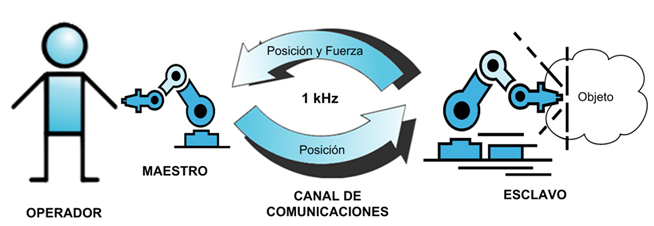
\includegraphics[scale=0.4]{FiguresP/MaestroEsclavo}
%\caption{Esquema de Control Maestro Esclavo}
%\label{fig:maestroesclavo}
%\end{figure}

%En la figura \ref{fig:maestro} se aprecia el dispositivo maestro del sistema de teleoperación, se muestran los ejes de movimiento.







\section{Sistema Esclavo}

Como sistema esclavo se tiene un brazo rob\'otico de seis grados de libertad con una pinza como efector final (ver figura \ref{Esclavo}), operado a base de actuadores hidr\'aulicos, sensores de presi\'on y posición.


\subsection{Sensores y Actuadores}

\begin{figure}
\centering
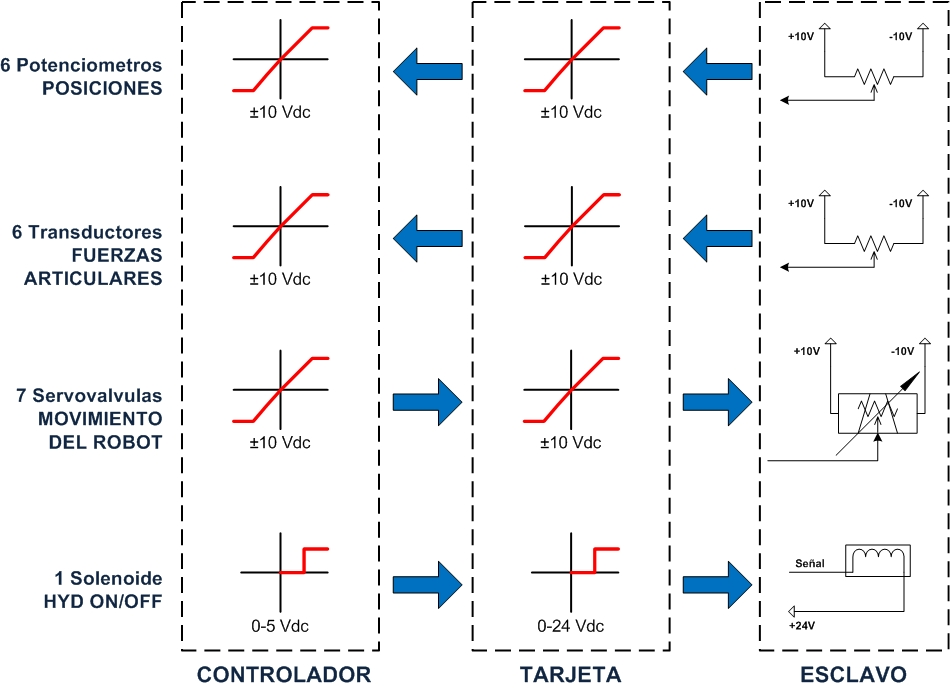
\includegraphics[scale=1]{FiguresP/EsquemaTarjetaEsclavo}
\caption{Esquema de la tarjeta de acondicionamiento de señales del dispositivo maestro}
\label{fig:EsquemaTarjetaEsclavo}
\end{figure}

\subsection*{Sensores}
La posición del robot se puede determinar gracias a los seis potenciómetros acoplados a cada grado de libertad. La fuerza ejercida por cada articulación y la pinza, con excepción de \textsc{Wrist Rotate} WR, es estimada por seis transductores de presión localizados en el colector de las válvulas. Las medidas obtenidas con estos transductores tienen suficiente precisión como para cerrar lazos de control \cite{Ferre2007a}. Las mediciones se realizan a través de un modulo de adquisición de datos conectado al bus del controlador de tiempo real, pasando primero por una etapa de acondicionamiento de señal (ver figura \ref{fig:TarjetaEsclavo})




\begin{figure}[htb]
\centering
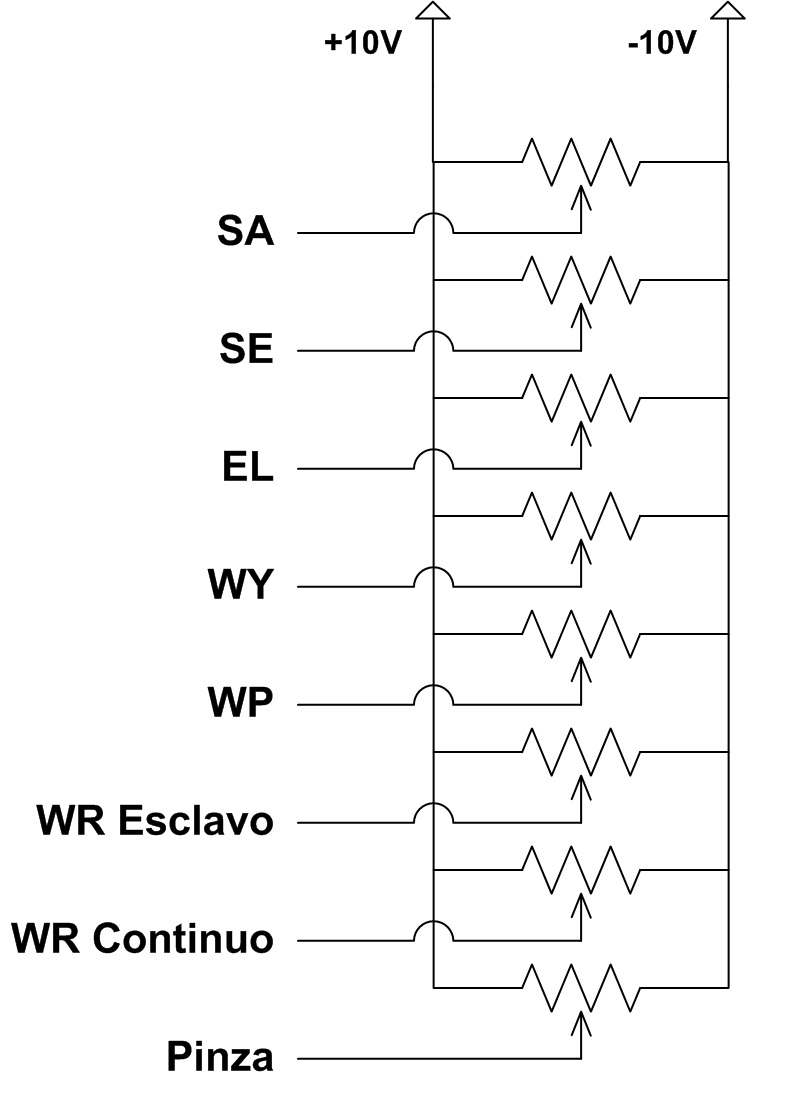
\includegraphics[scale=0.4]{FiguresP/Potenciometros}
\caption{Potenci\'ometros para medir la posición angular de cada una de las articulaciones}
\label{fig:potenciometros}
\end{figure}


\begin{figure}[htb!]
\centering
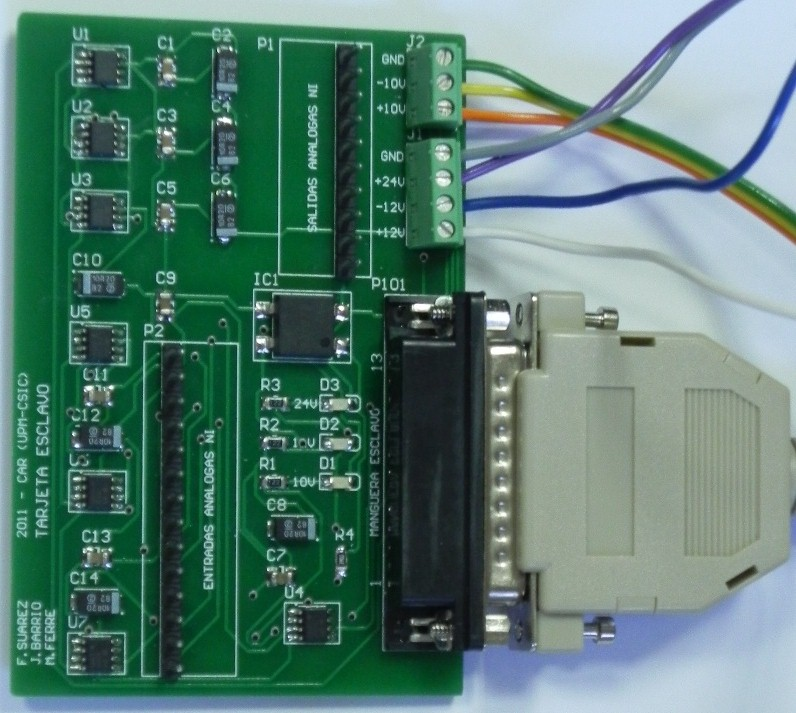
\includegraphics[scale=0.9]{FiguresP/TarjetaEsclavo}
\caption{Tarjeta del de acondicionamiento de señal del dispositivo Esclavo}
\label{fig:TarjetaEsclavo}
\end{figure}



\subsection*{Actuadores}
Cuenta con un conjunto de cilindros hidráulicos gobernados por  siete servoválvulas reguladoras de caudal que permiten regular el movimiento, además de una electroválvula que suministra la presión hidráulica al manipulador. La distribución de los actuadores permiten tres movimientos de brazo, tres movimientos de muñeca y la función de agarre de la pinza. Todos los movimientos, con excepción de WR y el cierre de la pinza, son trasmitidos utilizando actuadores tipo piñón - cremallera. El actuador de WR esta compuesto por un pistón tipo motor junto a una reductora con lo cual es posible realizar la rotación continua. Un pistón es utilizado para abrir y cerrar la pinza. 






\subsection{Cinemática Directa}

Es un manipulador del tipo antropomórfico de seis grados de libertad con una muñeca esférica con los siguientes parámetros de Denavit-Hartenberg

\begin{figure}[htb!]
\centering
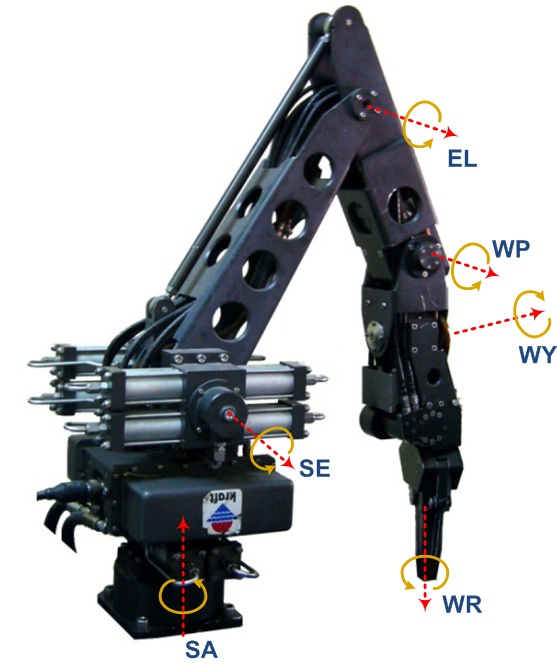
\includegraphics[scale=0.45]{FiguresP/EsclavoKraft}
\caption{Robot Esclavo }
\label{Esclavo}
\end{figure}



\begin{table}[htb!]
\caption{Parámetros de Denavit-Hartenberg para el robot esclavo GRIPS}
\centering
\label{tab:dhslave}
\begin{tabular}{ c c c c c }
 \hline
 Articulación & $a_i$ & $\alpha_i$ & $d_i$ & $\theta_i$ \\
 \hline
 1-SA 			& 0      & $-\frac{\pi}{2}$  & $l_1$     & $q_1$\\
 2-SE 			& $l_2$	 & 0                 & 0     & $q_2$\\
 3-EL 			& $l_3$	 & 0				    & 0     & $q_3$\\
 4-WP 			& $l_4$  & $\frac{\pi}{2}$   & 0     & $q_4$\\
 5-WY 			& 0      & $\frac{\pi}{2}$   & 0     & $q_5+\frac{\pi}{2}$\\
 6-WR 			& 0		 & 0                 & $l_6$     & $q_6$\\
 \hline
\end{tabular}
\end{table}



A partir de los parámetros de la tabla \ref{tab:dhslave} se obtiene una matriz de transformación sustituyendo  en la matriz de la ecuación \ref{dh}. Adicionalmente la figura \ref{fig:diaGrips} muestra un esquema con dichos parámetros.

\begin{equation}
^{i}A_{i-1}=\begin{pmatrix}
c\theta_i & -c\alpha_i s\theta_i & s\alpha_i s\theta_i & a_ic\theta_i\\
s\theta_i & c\alpha_i c\theta_i & -s\alpha_i c\theta_i & a_is\theta_i\\
0 & s\alpha_i & c\alpha_i & d_i\\
0 & 0 & 0 & 1
\end{pmatrix}
\label{dh}
\end{equation}


La posición y orientación del efector final con respecto al sistema fijo de la base se puede obtener multiplicando las matrices como se puede ver en la ecuación 

\begin{equation}
^{i}T_{0}=^{1}A_{0} \cdot ^{2}A_{1} \cdot  ^{3}A_{2} \cdot \cdots \cdot ^{6}A_{5} 
\end{equation}


A partir de estos parámetros se pueden obtener las matrices de rotación y de traslación para posteriormente calcular la cinemática directa e inversa del manipulador A partir de las matrices de transformación homogénea se obtiene la cinemática directa del robot antropomórfico de seis GDL. Existen distintos métodos para determinar la cinemática inversa, uno de ellos es multiplicando las matrices de rotación de cada eslabón si es revoluta o la matriz de traslación si es prismático. Otra opción para robots más complejos es el procedimiento de Denavit- Hartenberg, a continuación se muestra el procedimiento para el cálculo a través de las matrices de rotación y traslación.





\begin{figure}[htb!]
\centering
\subfigure{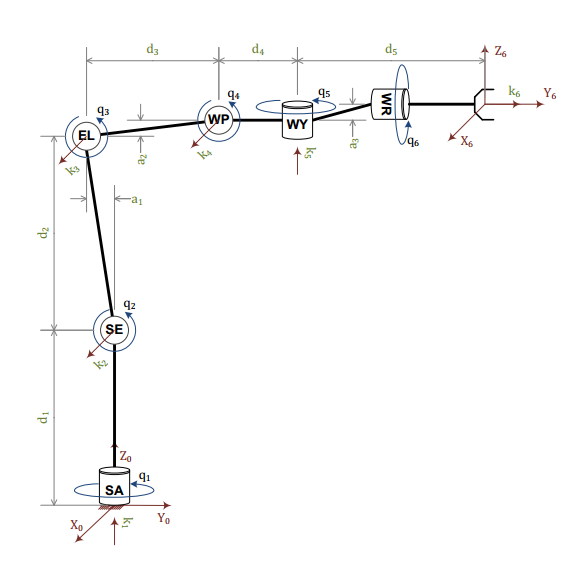
\includegraphics[scale=0.8]{FiguresP/DiagramaGrips}}
\subfigure{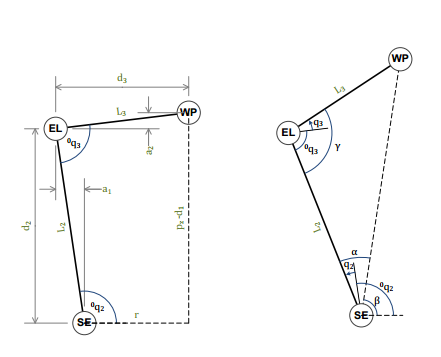
\includegraphics[scale=0.8]{FiguresP/DiagramaGrips2}}
\caption{Diagrama del Robot Grips}
\label{fig:diaGrips}
\end{figure}







%Given the special kinematic configuration of the MasterFinger 3, the use of the Denavit- Hartenberg convention [? ] would require dummy links to overcome the constraints that have to be met between coordinate frames. Specically, it would require a total of 14 joints for each finger when they only have 7.

%As an alternative, the displacement matrices approach proposed in [? ] can be used. This method can deal with any robot configuration without adding dummy links because it requires knowing the transformation (position and orientation) T0 of the robot end- efector at its home position (qi = 0 ∀ i), identifying the direction vector ki of the joint axis and selecting any point pi over the axis for all i.


También se presenta el método de matrices de desplazamiento \cite{barrientos2012modelado} como alternativa al método de Denavit y Hartenberg que puede trabajar sin la necesidad de añadir eslabones ficticios. Solo requiere conocer la transformación de la posición (posición y orientación) de $T_0$ del efector final del robot y su posición inicial, ($q_i=0 \forall i$), identificando la dirección del vector $\vec{k_i}$ del eje del eslabón y seleccionando algún punto $\vec{P_i}$ sobre el eje para todo $i$. Siendo $T_0$ la matriz de transformación, $q_i$ el i-\'esimo grado de libertad del robot y $\vec{k_i}$ el eje z del i-\'esimo eslabón. En el cuadro \ref{tab:dhslave} y en la figura 



%De manera similar al método de Denavit-Hartenberg \cite{hartenberg1964kinematic}, el método de matrices de desplazamiento
A continuación se presenta el algoritmo para encontrar el modelo cinemático directo usando matrices de desplazamiento.

\subsection{Modelo Cinemático Directo mediante Matrices de Desplazamiento}
\begin{itemize}
\item[D-1] Situando al robot en la posición cero ($q_i=0, \forall i$) encontrar la expresión de la matriz de transformación homogénea $T_0$ que localiza al extremo del robot referido al sistema de la base.

\item[D-2]
Para la misma posición del robot y para cada grado de libertad $q_i$ obtener la matriz de desplazamiento $D_i$, para ello:

\item[D-2.1]
    Identificar el vector unitario $\vec{k_i}$ del eje de la articulación expresado en las coordenadas del sistema de la base.

    

     \item[D-2.2] Seleccionar cualquier punto $\vec{P_i}$ del eje de la articulación

    \item[D-2.3] La matriz de desplazamiento asociada a ese grado de libertad, vendrá dada por\\
$$
D_i=\begin{pmatrix}
I & \vec{k_i}q_i\\
0 & 1
\end{pmatrix} 
$$
si el GDL es de traslación. O por\\
$$
D_i=\begin{pmatrix}
R_i & (I-R_i)\vec{p_i}\\
0 & 1
\end{pmatrix} 
$$
si el GDL es de rotación.\\

Siendo $I$ matriz identidad de dimensión 3 y la matriz $R_i$\\
\begin{center}


$R_i=I\cos{q_i}+\vec{k_i}\vec{k_i}^{T}(1-\cos{q_i})+skew(\vec{k_i})\sin{q_i}$\\
\end{center}
El operador \textbf{$skew$} es el que a cada vector $\vec{k}=(k_x,k_y,k_z)$ asocia la matriz antisimétrica.

$$skew(\vec{k})=\begin{pmatrix}
0 & -k_z & k_y\\
k_z & 0 & -k_x\\
-k_y & k_x & 0\\ 
\end{pmatrix}
$$
    
\item[D-3] El modelo cinemático directo \textsc{MCD} se tiene como el producto
$$
T_n=(\prod_{i=1}^n\mathbf{D_i})\mathbf{T_0}
$$

\end{itemize}

%\begin{algorithm}[H]  
% \KwData{situando al robot en la posición cero %($q_i=0, \forall i$) encontrar la expresión de la %matriz de transformación homogenea $T_0$ que se %localiza en el extremo del robot referido al sistema %de la base}
% \KwResult{how to write algorithm with \LaTeX2e }
% initialization\;
% \While{not at end of this document}{
%  read current\;
%  \eIf{understand}{
%   go to next section\;
%   current section becomes this one\;
%   }{
%   go back to the beginning of current section\;
%  }
% }
% \caption{Algoritmo para la obtención del modelo %cinemático del Robot mediante las Matrices de %Desplazamiento}
%\end{algorithm}


A continuación se presenta el código en Matlab que implementa lo anteriormente explicado.
\begin{lstlisting}
function T=MCD_MD (kk, pp, TO,tipo,n)
% kk(3,n) coordenadas del vector director del eje de la articulacion expresadas en {SO}, 
con el robot situado en qi=0
% pp(3,n) coordenadas de un punto del eje de la articulacion expresadas en {SO}, 
con el robot situado en qi=0
% TO (4,4) MTH del sistema de coordenadas del extremo {Sn} expresado en {SO},
 con el robot situado en cero qi = 0
% tipo(l,n) vale 0 si el gdl es de rotacion y 1 si es de traslacion
% n: numero de gdl
syms ql q2 q3 q4 q5 q6 real;
qq=sym([ql, q2, q3, q4, q5, q6]);
I=T0;
I=eye(3);
for i=n:-1:1
	k=kk (i,:)'; 	p=pp (i, :) ';q	=qq (i);
	if tipo(i)==0
		K=[0 -k(3) k(2);k(3) 0 -k(l);-k(2) ..
		k(l) 0];
		R=I*cos(q)+k*k'*(1-cos(q))+K*sin(q);
		D=[R, (I-R) *p; [0 0 0 1] ]
	else
		D=[eye (3) ,w*q; [0 0 0 1] ;
	end
I=simple(D*T);
end
end
 \end{lstlisting}  







\begin{table}[htb!]
\centering
\caption{Parámetros del método de matrices de desplazamiento para el robot GRIPS}
\label{tab:desplazamientoGrips}
\begin{tabular}{c c c}
\hline \\
Eje & Vector director $\vec{k_i}$ & Punto cualquiera en el eje de $\vec{P_i}$ \\
1				& $[0,0,1] $ &  $[0,0,0]$\\
2				& $[1,0,0] $ &  $[0,0,d_1]$\\
3				& $[1,0,0] $ &  $[0,-a_1,d_1+d_2]$\\
4				& $[1,0,0] $ &  $[0,-a_1+d_3,d_1+d_2+a_2]$\\
5				& $[0,0,1] $ &  $[0,-a_1+d_3+d_4,d_1+d_2+a_2]$\\
6				& $[0,1,0] $ &  $[-a_4,-a_1+d_3+d_4+d_5,d_1+d_2+a_2+d_3]$\\
\hline
\end{tabular}
\end{table}






En la ecuación \ref{eq:fkgrips} puede verse la matriz de desplazamiento para la cinemática directa del manipulador GRIPS y en la tabla \ref{tab:desplazamientoGrips} los valores a los que se hace referencia.
\begin{equation}
\label{eq:fkgrips}
T_0=\begin{pmatrix}
1 & 0 & 0 & -a_4\\
0 & 1 & 0 & -a_1+d_3+d_4+d_5\\
0 & 0 & 1 & d_1 +d_2+a_2+a_3\\
0 & 0 & 0 & 1  
\end{pmatrix}
\end{equation}

%Similar to the Denavit-Hartenberg  convention [? ], the displacement matrices method can be systematically implemented, see Algorithm 3.1. Placing the robot at its home position (qi = 0 ∀ i), and the homogeneous transformation T0 that locates the robot's end-efector reference frame relative to the base frame. In the same position and for each DoF qi obtain the displacement matrix Di : ˆ Identify the joint axis direction vector ki relative to the base frame. ˆ Select any point pi over the joint axis.



También puede utilizarse el método de matrices de desplazamiento en la obtención de la cinemática inversa, haciendo algunas simplificaciones para mantener expresiones mas claras:

$$
S_\theta=\sin\theta
$$

$$
C_\theta=\cos\theta
$$

$\mathbf{^{0}FK_{3}}$ La matriz de cinemática directa de los primeros tres GDL.

\begin{equation}
T_0=\begin{pmatrix}
1 & 0 & 0 & 0\\
0 & 1 & 0 & -a_1+d_3\\
0 & 0 & 1 & d_1+d_2+a_2\\
0 & 0 & 0 & 1  
\end{pmatrix}
\end{equation}


cuyos parametros pueden verse en la tabla \ref{tab:f3gdl}

\begin{table}[htb!]
\centering
\label{tab:f3gdl}
\caption{Parámetros del método de matrices de desplazamiento para los primeros tres GDL del robot GRIPS}
\begin{tabular}{c c c}
\hline \\
Eje & Vector director $\vec{k_i}$ & Punto cualquiera en el eje de $\vec{P_i}$ \\
1				& $[0,0,1] $ &  $[0,0,0]$\\
2				& $[1,0,0] $ &  $[0,0,d_1]$\\
3				& $[1,0,0] $ &  $[0,-a_1,d_1+d_2]$\\
\hline
\end{tabular}
\end{table}


obteniendo la siguiente matriz de transformación

%\begin{equation}
%^{0}T_3=\begin{pmatrix}
%c_1 & -c_{2+3} s_1  & s_{2+3}S_1   &  s_1(−d_3 c_{2+3} + a_2 s_{2+3} + a_1 c_2 + d_2 s_2 )\\
%s_1 &  c_{2+3} c_1  & -s_{2+3}C_1  & -c_1(-d_3 c_{2+3} + a_2 s_{2+3} + a_1 c_2 + d_2 s_2 )\\
%0   &  s_{2+3}      & c_{2+3}      & d_1 + a_2 c_{2+3} + d_3 s_{2+3} + d_2 c_2 + -a_1 s_2 \\
%0   &       0       &     0        &   1        
%\end{pmatrix}
%\end{equation}


Para los tre ultimos GDL (muñeca esferica) se tiene la matriz en la ecuación \ref{ec:fkwrist} $\mathbf{^{3}FK_6}$




\begin{equation}
\mathbf{T_0}=\begin{pmatrix}
1 & 0 & 0 & -a_4\\
0 & 1 & 0 & d_4+d_5\\
0 & 0 & 1 & a_3\\
0 & 0 & 0 & 1

\end{pmatrix}
\end{equation}



\begin{table}[htb!]
\centering
\label{tab:l3gdl}
\caption{Parámetros del método de matrices de desplazamiento para los últimos tres GDL del robot GRIPS}
\begin{tabular}{c c c}
\hline \\
Eje & Vector director $\vec{k_i}$ & Punto cualquiera en el eje de $\vec{P_i}$ \\
4				& $[1,0,0] $ &  $[0,0,0]$\\
5				& $[0,0,1] $ &  $[0,d_4,0]$\\
6				& $[0,1,0] $ &  $[-a_4,0,a_3]$\\
\hline
\end{tabular}
\end{table}


\begin{equation}
\label{ec:fkwrist}
\mathbf{^{6}T_3}=\begin{pmatrix}
n_x & o_x & a_x & p_x\\
n_y & o_y & a_y & p_y\\
n_z & o_z & a_z & p_z\\
0   & 0   & 0 & 1
\end{pmatrix}
\end{equation}




\begin{minipage}{0.9\textwidth}
\begin{tabular}{l l}


$n_x=C_5 C_6$ 				& \hspace{2cm} $a_x=C_5 S_6$\\
$n_y=S_4 S_5 +  C_4 C_6 S_5$	& \hspace{2cm} $a_y=-C_6 S_4 + C_4 S_5 S_6$\\
$n_z=-C_4 S_6 + C_6 S_4 S_5$ & \hspace{2cm} $a_z=C_4 C_6 + S_4 S_5 S_6$\\
$o_x=-S_5$ 					& \hspace{2cm} $p_x=-a_4 C_5 -d_5 S_5$\\
$o_y=C_4 C_5$ 				& \hspace{2cm} $p_y=d_4 C_4 -a_3 S_4 + d_5 C_4 C_5 -a_4 C_4 S_5$\\
$o_z=C_5 S_4$ 				& \hspace{2cm} $p_z=a_3 C_4 d_4 S_4  + d_5 C_5 S_4 -a_4 S_4 S_5$\\
\end{tabular}
\end{minipage}








%%A continuación se muestran las matrices de rotación y traslación que corresponden al robot planar de dos grados de libertad. Para obtener las coordenadas cartesianas hay que multiplicar las matrices de trasformación homogénea y evaluarlas en los puntos de las coordenadas articulares.\\
%
%
%\begin{eqnarray}
%R_{0}^{1}=\begin{pmatrix}
%\cos q_1 &  -\sin q_1 & 0 & 0\\
%\sin q_1 &   \cos q_1 & 0 & 0\\
%0        & 0          & 1 & 0\\
%0        & 0          & 0 & 1
%\end{pmatrix} \\ 
%T_{0}^{1}=\begin{pmatrix}
%1 & 0 & 0 & l1\cos(q1)\\
%0 & 1 & 0 & l1\sin(q1)\\
%0 & 0 & 1 & 0\\
%0 & 0 & 0 & 1
%\end{pmatrix} \\
%R_{1}^{2}=\begin{pmatrix}
%\cos q_2 &  -\sin q_2 & 0 & 0\\
%\sin q_2 &   \cos q_2 & 0 & 0\\
%0        & 0          & 1 & 0\\
%0        & 0          & 0 & 1
%\end{pmatrix} \\ 
%T_{1}^{2}=\begin{pmatrix}
%1 & 0 & 0 & l2\cos(q2)\\
%0 & 1 & 0 & l2\sin(q2)\\
%0 & 0 & 1 & 0\\
%0 & 0 & 0 & 1
%\end{pmatrix} \\
%A_0^{2}=R_0^{1} T_0^{1} R_1^{2} T_1^{2} 
%\end{eqnarray}
%
%Para  calcular la cinemática directa se introducen en un \textbf{Script de MATALB} las matrices de traslación y rotación del mecanismo, y se proponen valores para $q_1,l_1 $ y $q_2,l_2 $ , como se puede ver a continuación:
%\begin{verbatim}
%q1=30;
%q2=45;
%l1=1;
%l2=1;
%t1=[[1 0 0 l1*cosd(q1)]
%    [0 1 0 l1*sind(q1)]
%    [0 0 1 0]
%    [0 0 0 1]]
%
%t2=[[cosd(q1) -sind(q1) 0 0]
%    [sind(q1) cosd(q1)  0 0]
%    [0 0 1 0]
%    [0 0 0 1]]
%
%
%t3=[[1 0 0 l2*cosd(q2)]
%    [0 1 0 l2*sind(q2)]
%    [0 0 1 0]
%    [0 0 0 1]]
%
%
%t4=[[cosd(q2) -sind(q2) 0 0]
%    [sind(q2) cosd(q2)  0 0]
%    [0 0 1 0]
%    [0 0 0 1]]
%\end{verbatim}
%Después podemos resolver el problema mediante el método de Denavit Hartenberg solo para comprobar nuestro resultado:
%
%\begin{tabular}{|c|c|c|c|c|}
%
%\hline 
%Articulación & $\theta$ & d & a & $\alpha$ \\ 
%\hline 
%1 & $q_1$ & 0 & $l_1$ & 0 \\ 
%\hline 
%2 & $q_2$ & 0 & $l_2$ & 0 \\ 
%\hline 
%\end{tabular} 


%
%
%\begin{verbatim}
%a01=[[cosd(q1) -sind(q1) 0 l1*cosd(q1)]
%    [sind(q1) cosd(q1) 0 l1*sind(q1)]
%    [0 0 1 0]
%    [0 0 0 1]]
%
%
%a12=[[cosd(q2) -sind(q2) 0 l2*cosd(q2)]
%    [sind(q2) cosd(q2) 0 l2*sind(q2)]
%    [0 0 1 0]
%    [0 0 0 1]]
%    
%T=t1*t2*t3*t4
%dh=a01*a12
%\end{verbatim}
%
%
%Como resultado tenemos:
%\begin{verbatim}
%T = 0.2588   -0.9659         0    1.1248
%    0.9659    0.2588         0    1.4659
%         0         0    1.0000         0
%         0         0         0    1.0000
%
%
%dh =0.2588   -0.9659         0    1.1248
%    0.9659    0.2588         0    1.4659
%         0         0    1.0000         0
%         0         0         0    1.0000
%
%\end{verbatim}
%Podemos observar el mismo resultado con lo que se concluye que se ha efectuado el procedimiento de  manera correcta. Se muestra también una representación gráfica del mecanismo en la figura


\subsection{Cinemática inversa}
Se tiene el siguiente conjunto de ecuaciones obtenidas del la figura \ref{fig:diaGrips} , las cuales describen las coordenadas articulares del robot, a partir de un punto dado en el espacio mediante relaciones geométricas simples para los tres primeros grados de libertad.

\begin{eqnarray}
 q_1=\arctan{\frac{P_y}{P_x}} \\ 
 r^{2}=P_x^{2}+P_y^{2}\\ 
 r^{2}=+P_2^{2}=l_2^{2}+l_3^{2}+l_2l_3\cos{q_3}\\ 
 \cos{q_3}=\frac{P_x^{2}+P_y^{2}+P_2^{2}-l_2^{2}-l_3^{2}}{2l_2l_3}\\ 
 \sin{q_3}=\sqrt{1-\cos^{2}{q_3}}\\ 
 q_3=\arctan{\frac{\sqrt{1-\cos^{2}{q_2}}}{\cos{q_3}}}\\ 
 q_2=\beta -\alpha\\ 
 \beta=\arctan{\frac{P_z}{r}}=\arctan{\frac{P_z}{\sqrt{P_x^{2}+P_y^{2}}}}\\ 
 \alpha=\arctan{\frac{l_2\sin{q_3}}{l_2+l_3 \cos{q_3}}}\\ 
 q_2=\arctan{\frac{P_z}{\sqrt{P_z^{2}}+P_y^{2}}}-\arctan{\frac{l_3\sin{q_3}}{l_2+l_3\cos{q_3}}}
\end{eqnarray}
Se observa que en la cinemática inversa pueden existir soluciones alternas. Debido a esto usamos la función \textbf{atan2} la cual nos arroja solo una de las posibles soluciones.\\
 
 
Para el caso de la orientación del efector final se tienen las siguientes ecuaciones obtenidas a partir de la ecuación \ref{ec:fkwrist} 




%La siguiente función en MATLAB recibe como entrada las coordenadas cartesianas del efector final del robot y devuelve las coordenadas articulares.
%\subsection{Desplazamiento lineal}
%Se creo la siguiente función en MatLab para el robot de dos grados de libertad
%\begin{verbatim}
%function Y=dosgdl(l2, l3, py, px)
%Cq3=(px^2+py^2-l2^2-l3^2)/(2*l2*l3)
%Sq3= sqrt(1-((Cq3)^2))
%q3= atand(Sq3/Cq3)
%Betha = atand(py/px)
%Alfa = atand((l3*sind(q3))/(l2+(l3*Cq3)))
%q2=Betha-Alfa
%%x2=[0 l2*cosd(q2)]
%%y2=[0.5 l2*sind(q2)]
%x3=[0 l2*cosd(q2) l3*cosd(q3+q2)+l2*cosd(q2)]
%y3=[0 l2*sind(q2) l3*sind(q3+q2)+l2*sind(q2)]
%Y=[x3;y3]
%%line(x2, y2);
%line(x3, y3);
%axis([0 5 0 5]); 
%\end{verbatim}
%
%
%
%
%Posteriormente se varía la trayectoria a seguir por el robot usando un ciclo for
%\begin{verbatim}
%clc, clear, close all
%l2=2;
%l3=1;
%xt=[];
%yt=[];
%px= []
%py= 2;
%for px=1:0.1:2.2
%
%Y= dosgdl(l2, l3, py, px);
%xt= Y(1);
%yt= Y(2);
%drawnow;
%pause(0.1);
%clf;
%end
%\end{verbatim}
%



















%\newpage
%\subsection{Ecuaciones dinámicas}
%Podemos modelar este sistema como un péndulo doble ver figura  en general el péndulo doble es un sistema compuesto por dos péndulos, con el segundo extremo colgando del primero, asumimos que se trata de dos péndulos simples, este sistema físico posee dos grados de libertad. su movimiento está gobernado por dos ecuaciones diferenciales ordinarias acopladas. Cabe mencionar que por encima de cierta energía el sistema es caótico. Para el modelado del sistema usamos el método de \textbf{Euler-Lagrange}, como se muestra a continuación.

%\subsection{Energía}
%
%La energía cinética puede expresarse como:
%\begin{eqnarray}
%T=\frac{1}{2}m_1(\dot{x}_1^{2}+\dot{y}_1^{2})+\frac{1}{2}m_2(\dot{x}_2^{2}+\dot{y}_2^{2})\\
%=\frac{1}{2}m_1 l_1^{2}\dot{\theta}_1^{2}+\frac{1}{2}m_2(l_1^{2}\dot{\theta}_1^{2}+l_2^{2}\dot{\theta}_2^{2} + 2l_1^{2} l_2^{2}\dot{\theta}_1^{2} \dot{\theta}_2^{2} \cos{(\theta_1-\theta_2)})
%\end{eqnarray}
%
%La energía potencial:
%\begin{eqnarray}
%V=m_1 g y_1 + m_2 g y_2\\
%=-(m_1 + m_2)gl_1 \cos\theta_1 -m_2gl_2 \cos\theta_2
%\end{eqnarray}
%Tenemos que la siguiente ecuación  según \textbf{Lagrange} es:
%\begin{equation}
%L=T-V
%\end{equation}
%Sustituyendo la energía cinética y potencial en la ecuación de \textbf{Lagrange} tenemos:
%\begin{equation}
%L=\frac{1}{2}m_1 l_1^{2}\dot{\theta}_1^{2}+\\
% \frac{1}{2}m_2(l_1^{2}\dot{\theta}_1^{2}+l_2^{2}\dot{\theta}_2^{2} + 2l_1^{2} l_2^{2}\dot{\theta}_1^{2} \dot{\theta}_2^{2} \cos{(\theta_1-\theta_2)})+(m_1 + m_2)gl_1 \cos\theta_1 +m_2gl_2 \cos\theta_2
%\label{lagrangiano}
%\end{equation}
%
%A partir de la ecuación \ref{lagrangiano} podemos obtener la ecuación del movimiento a partir de las ecuaciones \ref{l1} y \ref{l2}:
%
%\begin{eqnarray}
%\frac{d}{dt}(\frac{\partial L}{\partial \dot{\theta}_1})-\frac{\partial L}{\partial \theta_1 } \label{l1}\\ 
%\frac{d}{dt}(\frac{\partial L}{\partial \dot{\theta}_2})-\frac{\partial L}{\partial \theta_2 } \label{l2}
%\end{eqnarray}
%
%\begin{flushleft}
%{ \fboxsep 12pt
%
%\begin{minipage}[t]{18cm}
%
%Haciendo las correspondientes derivadas parciales y ordinarias llegamos a las ecuaciones de movimiento:
%
%\begin{align}
%(m_1+m_2)l_1^{2} \ddot{\theta}_1+ m_2\ddot{\theta}_2 l_1 l_2 \cos{(\theta_1-\theta_2)}-m_2\dot{\theta}_2 l_1 l_2(\theta_1 - \theta_2)\sin{(\theta_1-\theta_2)} +m_2\dot{\theta}_1 \dot{\theta}_2 l_1 l_2 \sin{(\theta_1 -\theta_2)}+ (m_1 + m_2) gl_1\sin{\theta_1} =0\\
%m_2l_2^{2}\ddot{\theta}_2 + m_2\ddot{\theta}_1 l_1 l_2 \cos{(\theta_1 - \theta_2)} -m_2 \dot{\theta}_1 l_1 l_2(\dot{\theta}_1-\dot{\theta}_2)\sin{(\theta_1-\theta_2)} -m_2\dot{\theta}_1\dot{\theta}_2 l_1 l_2 \sin{(\theta_1- \theta_2)}+m_2gl_2\sin \theta_2= 0
%\end{align}
%\end{minipage}
% }
%\end{flushleft}




\newpage
\subsection{Espacio de Trabajo}

En la figura \ref{fig:gripsworkspace} se muestra el espacio de trabajo del manipulador esclavo GRIPS


\begin{figure}[htb!]
\subfigure[\'Area de trabajo en el plano XZ del robot esclavo]{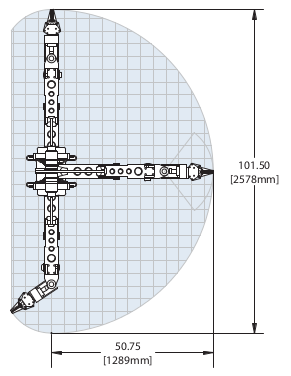
\includegraphics[scale=0.5]{FiguresP/grips6}}
\subfigure[\'Area de trabajo en el plano XY del robot esclavo]{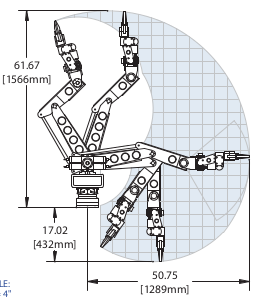
\includegraphics[scale=0.6]{FiguresP/grips5}}
\subfigure[Robot esclavo GRIPS]{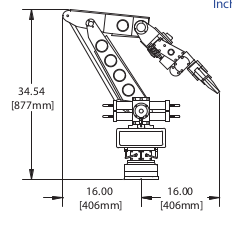
\includegraphics[scale=0.6]{FiguresP/grips1}}
\caption{Espacio de trabajo del robot esclavo Grips}
\label{fig:gripsworkspace}
\label{RobotGrips}
\end{figure}


\section{Señales del Robot Esclavo}
En la tabla \ref{tab:signalsSlave} se describen las señales del manipulador esclavo.
\begin{sidewaystable}[htbp]
  \centering
  \caption{Listado de señales del robot esclavo}
    \begin{tabular}{lllccccc}
    \toprule
    \multicolumn{1}{c}{\multirow{2}{*}{\textbf{TAG}}} & \multicolumn{1}{c}{\multirow{2}{*}{\textbf{ORIGEN}}} & \multicolumn{1}{c}{\multirow{2}{*}{\textbf{DESCRIPCIÓN}}} & \multicolumn{1}{c}{\multirow{2}{*}{\textbf{TIPO SEÑAL}}} & \multicolumn{4}{c}{\textbf{SEÑAL}} \\  
  &  &  & & \textbf{DI} & \textbf{DO} & \textbf{AI} & \textbf{AO} \\
    \midrule
  	SLA-VSA & Esclavo, Servo-Valvula SA & Salida Analógica, $\pm$10V, 200mA & Comando &       &       &       & 1 \\
    SLA-VSE & Esclavo, Servo-Valvula SE & Salida Analógica, $\pm$10V, 200mA & Comando &       &       &       & 1 \\
    SLA-VEL & Esclavo, Servo-Valvula EL & Salida Analógica, $\pm$10V, 200mA & Comando &       &       &       & 1 \\
    SLA-VWY & Esclavo, Servo-Valvula WY & Salida Analógica, $\pm$10V, 200mA & Comando &       &       &       & 1 \\
    SLA-VWP & Esclavo, Servo-Valvula WP & Salida Analógica, $\pm$10V, 200mA & Comando &       &       &       & 1 \\
    SLA-VWR & Esclavo, Servo-Valvula WR & Salida Analógica, $\pm$10V, 200mA & Comando &       &       &       & 1 \\
    SLA-VGRIP & Esclavo, Servo-Valvula Gripper & Salida Analógica, $\pm$10V, 200mA & Comando &       &       &       & 1 \\
    SLA-PSA & Esclavo, Potenciómetro SA & Valor de Voltaje $\pm$10V & Medida &       &       & 1     &  \\
    SLA-PSE & Esclavo, Potenciómetro SE & Valor de Voltaje $\pm$10V & Medida &       &       & 1     &  \\
    SLA-PEL & Esclavo, Potenciómetro EL & Valor de Voltaje $\pm$10V & Medida &       &       & 1     &  \\
    SLA-PWP & Esclavo, Potenciómetro WP & Valor de Voltaje $\pm$10V & Medida &       &       & 1     &  \\
    SLA-PWY & Esclavo, Potenciómetro WY & Valor de Voltaje $\pm$10V & Medida &       &       & 1     &  \\
    SLA-PWR & Esclavo, Potenciómetro WR & Valor de Voltaje $\pm$10V & Medida &       &       & 1     &  \\
    SLA-TSA & Esclavo, Transductor SA & Valor de Voltaje $\pm$10V & Medida &       &       & 1     &  \\
    SLA-TSE & Esclavo, Transductor SE & Valor de Voltaje $\pm$10V & Medida &       &       & 1     &  \\
    SLA-TEL & Esclavo, Transductor EL & Valor de Voltaje $\pm$10V & Medida &       &       & 1     &  \\
    SLA-TWP & Esclavo, Transductor WP & Valor de Voltaje $\pm$10V & Medida &       &       & 1     &  \\
    SLA-TWY & Esclavo, Transductor WY & Valor de Voltaje $\pm$10V & Medida &       &       & 1     &  \\
    SLA-TGR & Esclavo, Transductor GR & Valor de Voltaje $\pm$10V & Medida &       &       & 1     &  \\
    SLA-HYD & Esclavo, Solenoide Principal & Electroválvula, +24V, 1A & Comando &       & 1     &       &  \\
    \midrule
    \multicolumn{4}{r}{\textbf{TOTAL}} & 0 & 1 & 12 & 7 \\
    \bottomrule
    \end{tabular}%
  \label{tab:signalsSlave}%
\end{sidewaystable}%








































\newpage
\section{Sistema Maestro}

\begin{figure}[htb!]
\centering
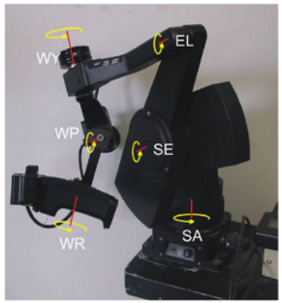
\includegraphics[scale=0.95]{FiguresP/Maestro}
\caption{Manipulador Maestro }
\label{fig:maestro}
\end{figure}

El robot maestro (ver figura \ref{fig:maestro}) es cinemáticamente similar al robot esclavo. Tiene tres grados de libertad para determinar la posición de la muñeca y tres m\'as para determinar su orientación. Como sensores de posición angular el sistema maestro cuenta con potenci\'ometros en cada una de las seis articulaciones. Las cinco primeras son actuadas eléctricamente para reflejar las fuerzas ejercidas en el robot esclavo. La pinza puede controlarse de manera proporcional pero sin realimentación por medio de un potenciometro. También cuenta con distintos botones para activar funciones como la rotación continua de la muñeca, bloqueo de la pinza y bloquear y continuar en la posición del esclavo y maestro.\\

Un botón ubicado en la base del maestro controla el encendido del sistema hidráulico, en el antebrazo  se encuentran tres LED que indican el estado de bloqueo de la pinza (\textit{Grip lock}), el modo de rotación de la muñeca (\textit{Cont wrist}), y el bloqueo de la posición del sistema (\textit{Halt}). Un LED ubicado al lado del botón para encender la hidráulica indica su estado (ver figura \ref{fig:leds}).



\begin{figure}[htb!]
\centering

\subfigure[Leds indicadores de estado]{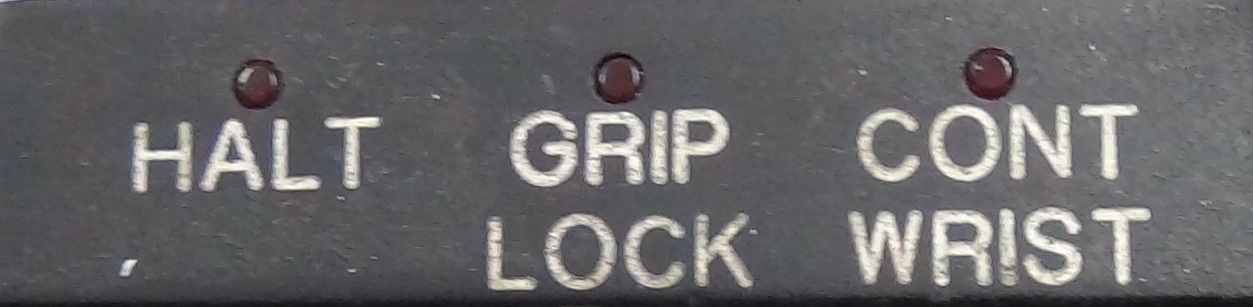
\includegraphics[scale=0.1]{FiguresP/leds}\label{fig:leds}}
\subfigure[Pulsador de hidráulica on/off]{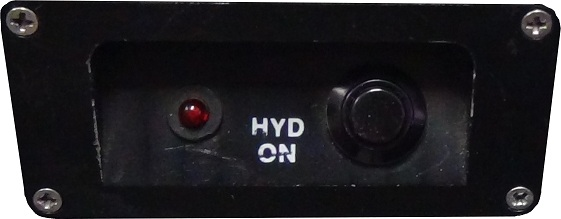
\includegraphics[scale=0.3]{FiguresP/PulsadorHyd}\label{fig:pulsadorhid}}
\subfigure[Detalle de la muñeca del dispositivo maestro]{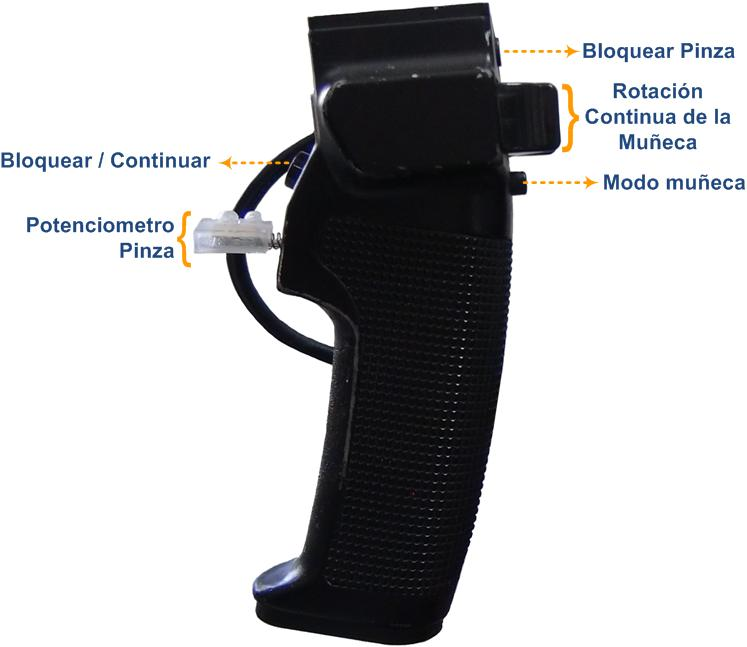
\includegraphics[scale=0.4]{FiguresP/Pulsadores}\label{fig:muñeca}}
\caption{Botones, LED y potenci\'ometros del maestro GRIPS}
\label{fig:leds}
\end{figure}








\newpage
\subsection{Sensores y Actuadores}

\begin{figure}[hbt!]
\centering
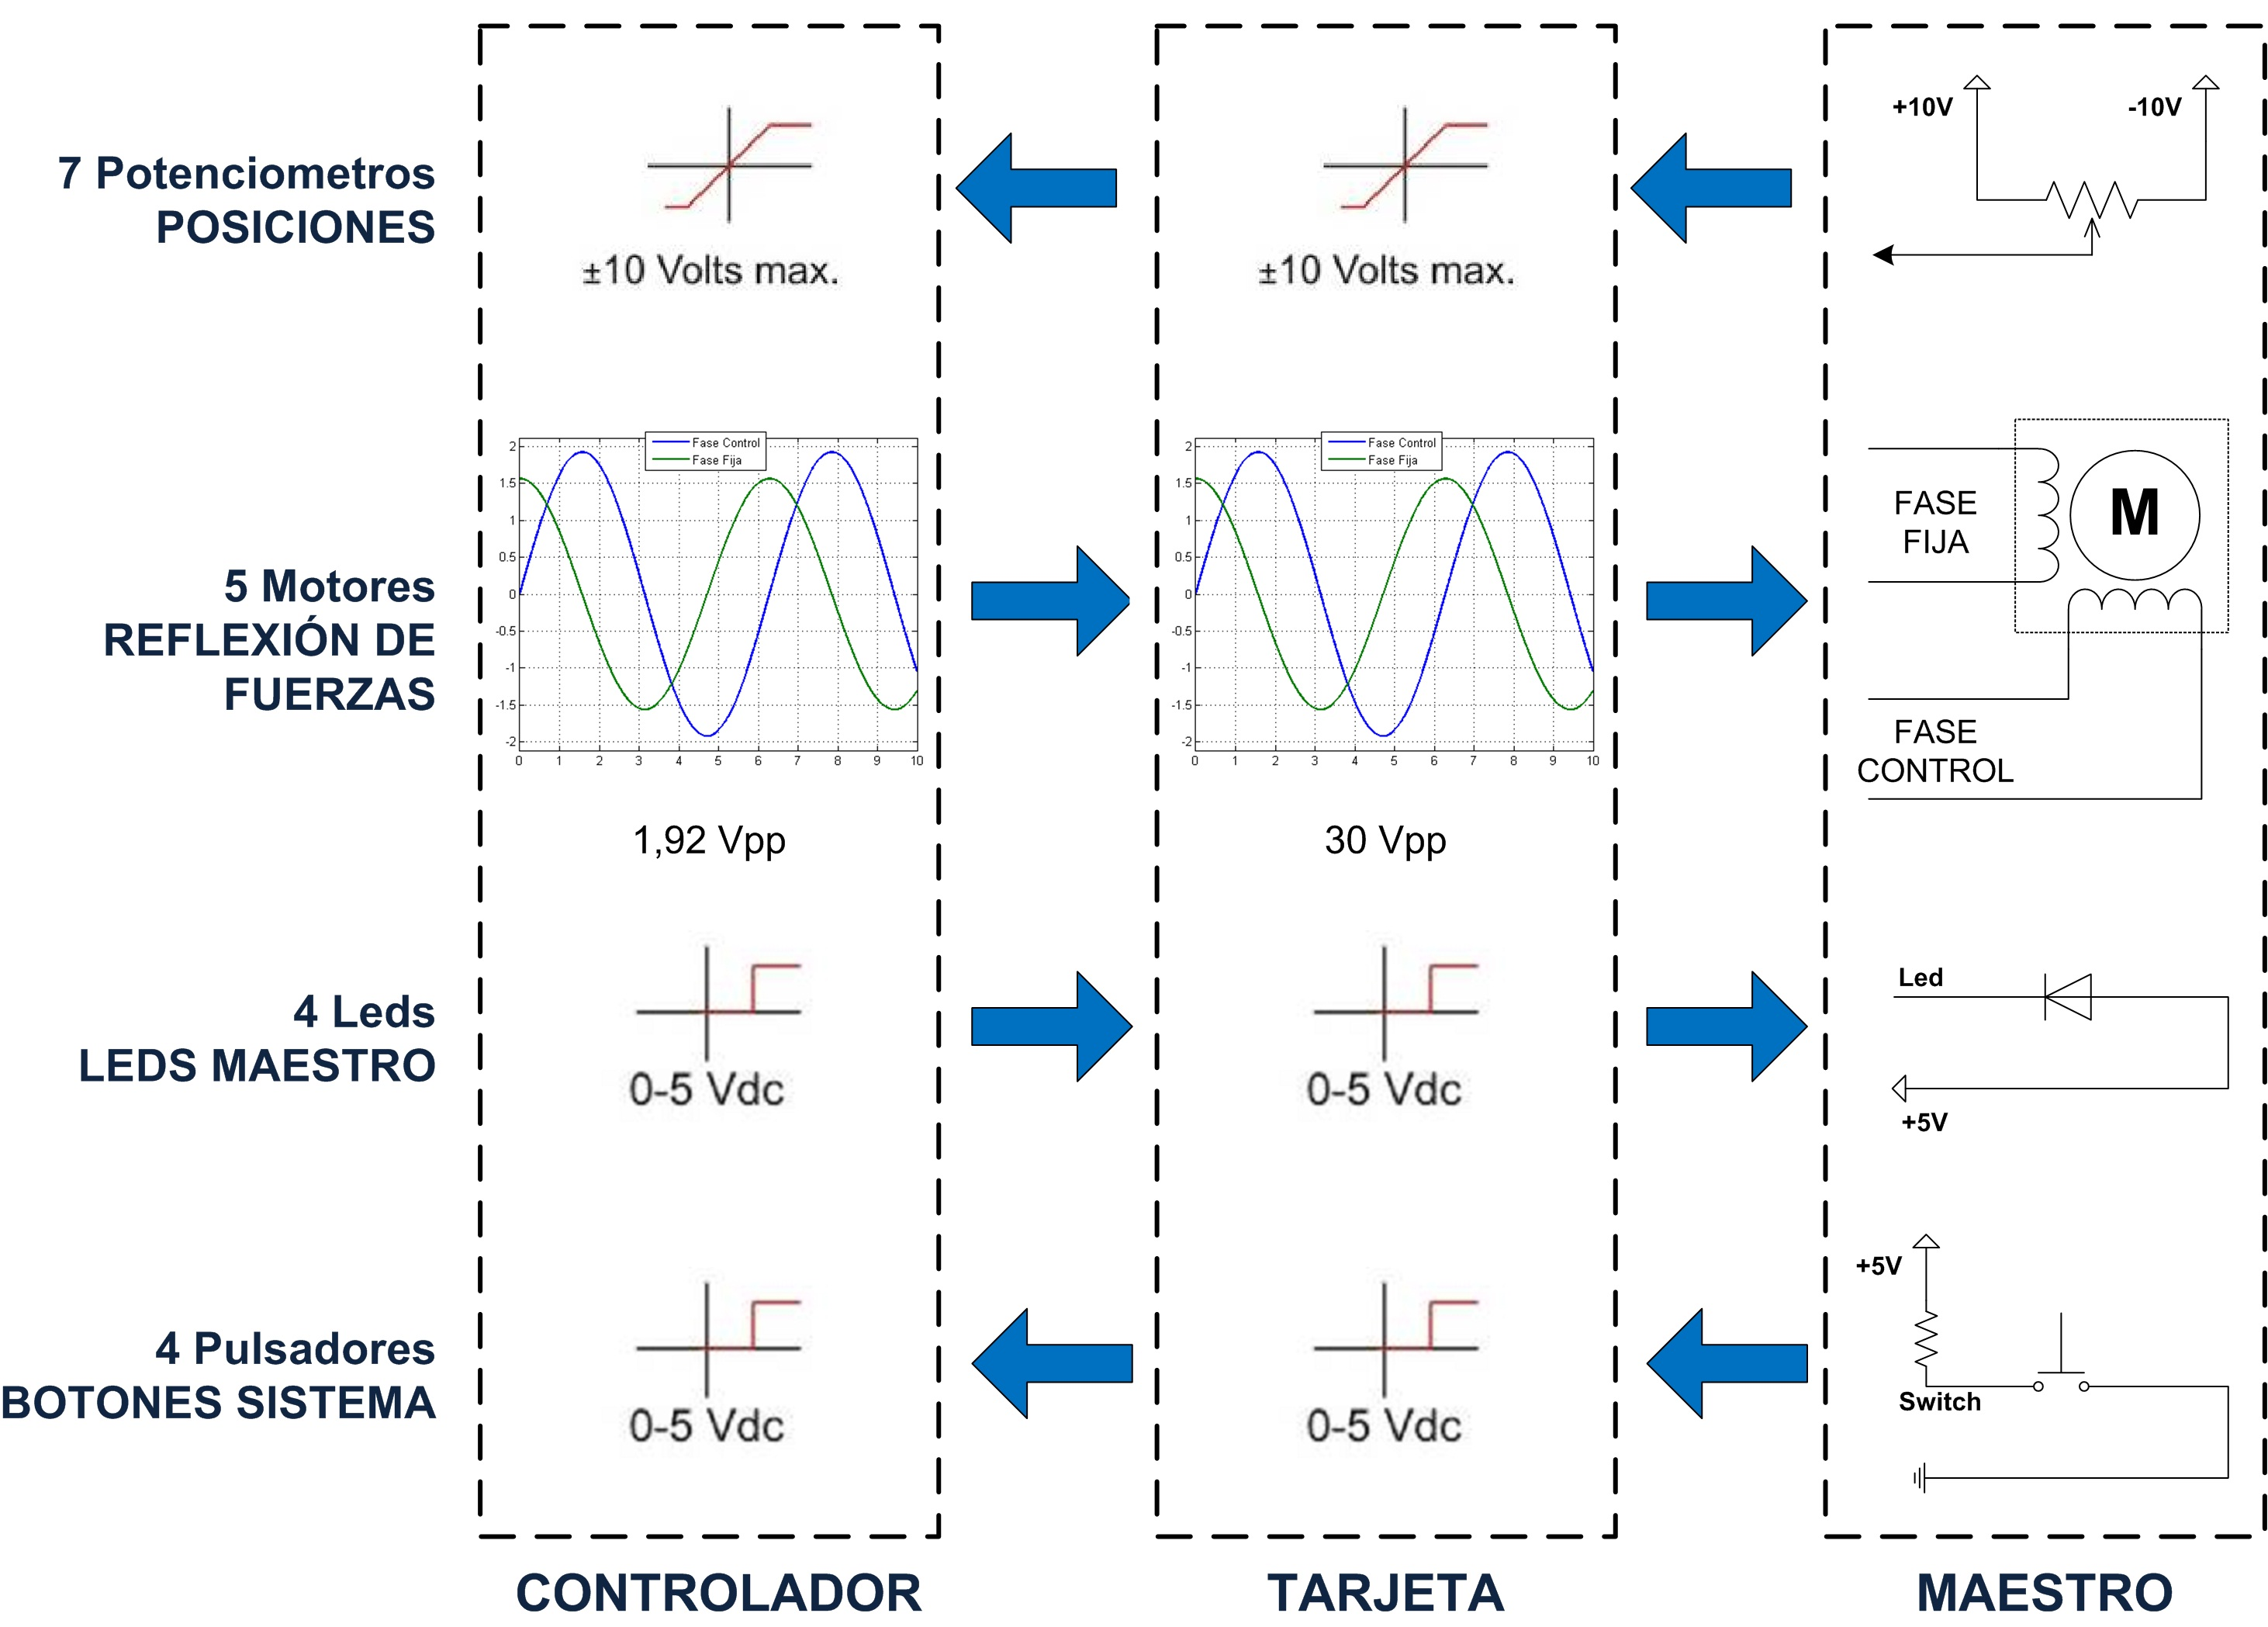
\includegraphics[scale=0.2]{FiguresP/EsquemaMaestroCard}
\caption{Tarjeta para Mediciones de Corriente}
\label{fig:TarjetaCorriente}
\end{figure}

\subsection*{Sensores}
El sistema maestro al igual que el sistema esclavo cuenta con poteni\'ometros para determianr las posiciones angulares de las articulaciones.




\subsection*{Actuadores}
Como puede observarse en la figura \ref{fig:motores}, el dispositivo maestro cuenta con cinco motores bif\'asicos de corriente alterna para realimentar la fuerza ejercida en el entorno remoto al operador. Para accionarlos son necesarias dos señales de corriente alterna(ver figura \ref{fig:señales}) que son generadas por el controlador de tiempo real y posteriormente amplificadas en una etapa de potenciab(ver figura \ref{fig:TarjetaMaestro}).  El sentido de rotación del motor depende de si la fase de control est\'a en adelanto o en atraso respecto a la fase fija. El par ejercido depende de la amplitud de ambas ondas.


\begin{figure}[htb!]
\centering
\subfigure[Señales de control para los motores del dispositivo maestro]{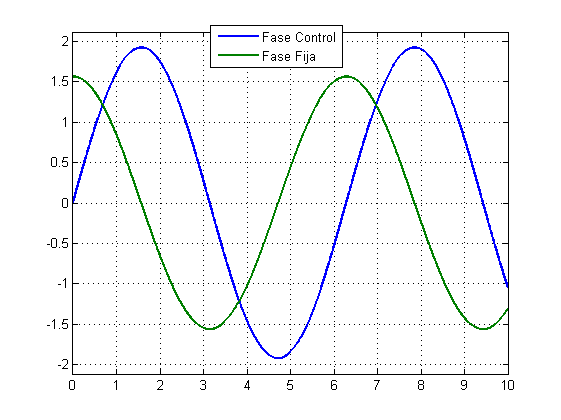
\includegraphics[scale=0.4]{FiguresP/entradaMotores}\label{fig:señales}}
\subfigure[Motores bifasicos utilizados para la realimentacion de fuerzas al operador]{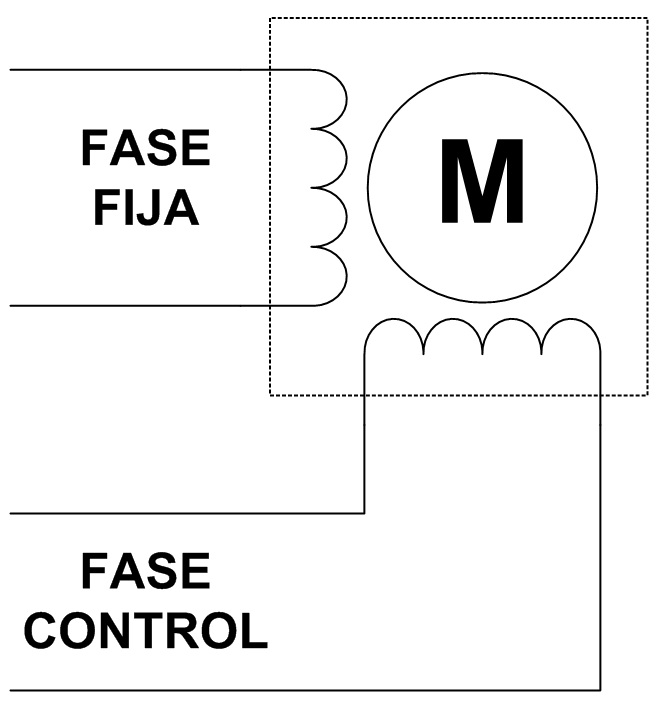
\includegraphics[scale=0.2]{FiguresP/MotorBifasico}\label{fig:motores}}
\caption{Esquema de los actuadores usados en el dispositivo maestro}
\end{figure}





\section*{Electrónica de Potencia}
Las señales de control son amplificadas en el circuito de la figura \ref{fig:etapaPotencia}.
\begin{figure}[htb!]
\centering
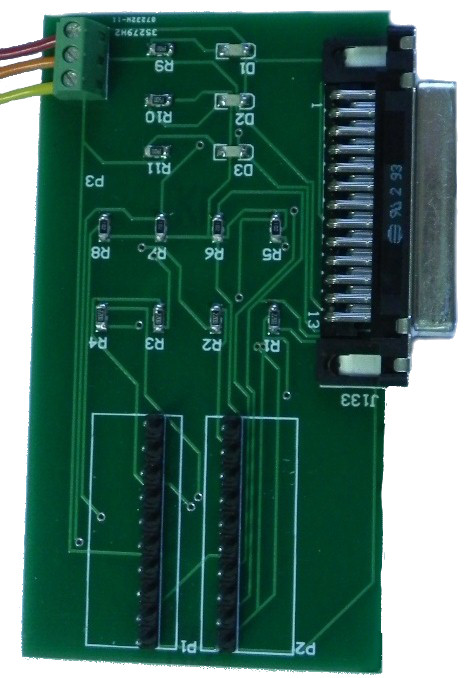
\includegraphics[scale=0.9]{FiguresP/TarjetaMaestro}
\caption{Tarjeta de entradas/salidas digitales y analógicas }
\label{fig:TarjetaMaestro}
\end{figure}


P

\begin{figure}[htb!]
\centering
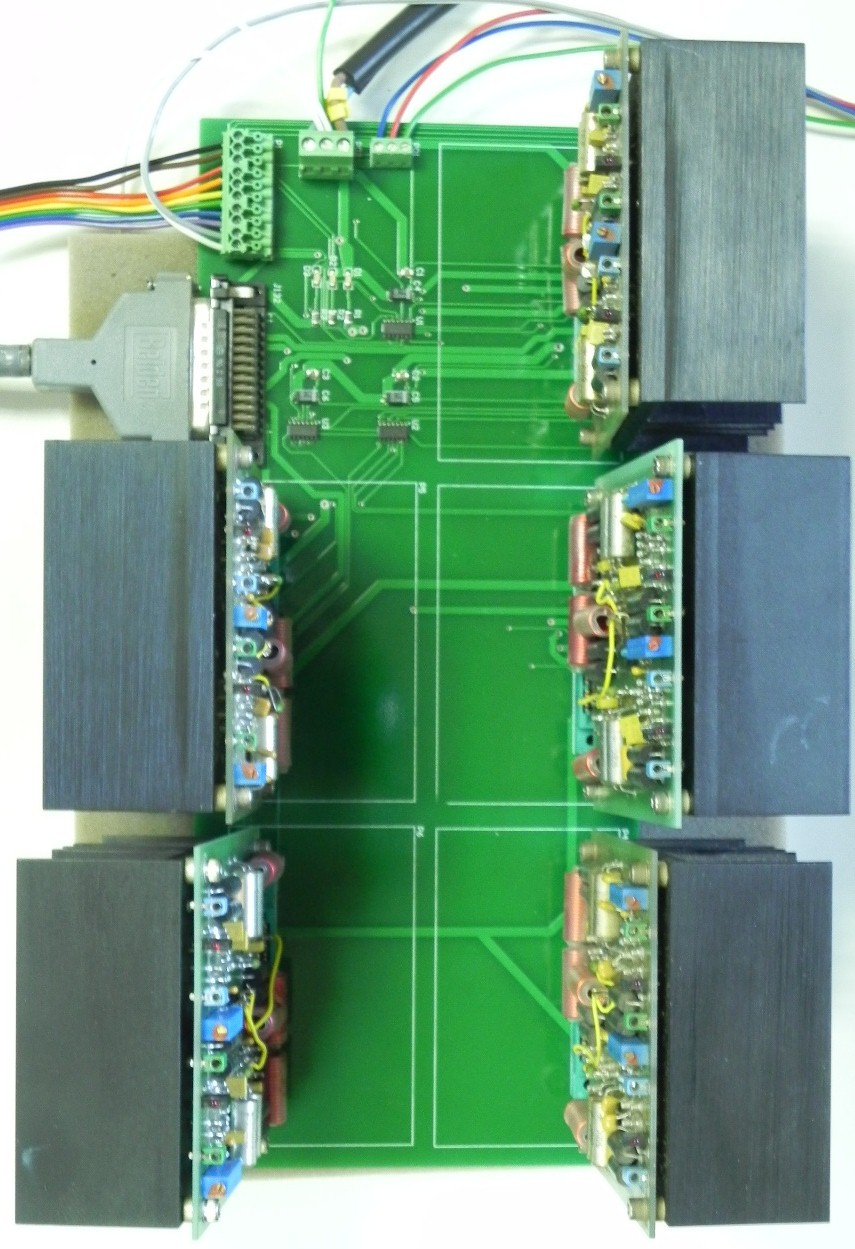
\includegraphics[scale=0.6]{FiguresP/TarjetaMotores}
\caption{Etapa de potencia de los motores}
\label{fig:etapaPotencia}
\end{figure}










%\subsection{Modelo Cinemático y Parámetros D-H}
%\begin{table}[]
%\centering
%\begin{tabular}{|c|c|c|c|c|}
% \hline
% \hline
% Articulación & $a_1$ & $\alpha_i$ & $d_i$ & $\theta_i$ \\
% \hline
% \hline
% 1 & 0      & $\frac{\pi}{2}$  & 0     & $\theta_1$\\
% 2 & $a_2$  & 0                & 0     & $\theta_1$\\
% 3 & 0      & $\frac{\pi}{2}$  & 0     & $\theta_1$\\
% 4 & 0      & $\frac{-\pi}{2}$ & $d_3$ & $\theta_1$\\
% 5 & 0      & $\frac{\pi}{2}$  & 0     & $\theta_1$\\
% 6 & 0      & 0                & $d_6$ & $\theta_1$\\
% \hline
% \hline
%\end{tabular}
%\caption{Parámetros D-H}
%\label{tab:MCD}
%\end{table}


%\subsection{Ecuaciones dinámicas}
%El Formalismo Lagrangiano presenta varias ventajas  en comparación con el método de Newton-Euler como lo son la fácil compresnión, ademas las matrices de inercia







%\subsection{Modelo Cinemático Inverso}



%\subsection{Espacio de Trabajo}





%Para el control LabView lenguaje gráfico de programación que permite 

%LabVIEW (acrónimo de Laboratory Virtual Instrumentation Engineering Workbench) es una plataforma y entorno de desarrollo para diseñar sistemas, con un lenguaje de programación visual gráfico. Recomendado para sistemas hardware y software de pruebas, control y diseño, simulado o real y embebido, pues acelera la productividad. El lenguaje que usa se llama lenguaje G, donde la G simboliza que es lenguaje Gráfico.

%Este programa fue creado por National Instruments (1976) para funcionar sobre máquinas MAC, salió al mercado por primera vez en 1986. Ahora está disponible para las plataformas Windows, UNIX, MAC y GNU/Linux. La última versión es la 2013, con la increíble demostración de poderse usar simultáneamente para el diseño del firmware de un instrumento RF de última generación, a la programación de alto nivel del mismo instrumento, todo ello con código abierto.

%Los programas desarrollados con LabVIEW se llaman Instrumentos Virtuales, o VIs, y su origen provenía del control de instrumentos, aunque hoy en día se ha expandido ampliamente no sólo al control de todo tipo de electrónica (Instrumentación electrónica) sino también a su programación embebida, comunicaciones, matemáticas, etc. Un lema tradicional de LabVIEW es: "La potencia está en el Software", que con la aparición de los sistemas multinúcleo se ha hecho aún más potente. Entre sus objetivos están el reducir el tiempo de desarrollo de aplicaciones de todo tipo (no sólo en ámbitos de Pruebas, Control y Diseño) y el permitir la entrada a la informática a profesionales de cualquier otro campo. LabVIEW consigue combinarse con todo tipo de software y hardware, tanto del propio fabricante -tarjetas de adquisición de datos, PAC, Visión, instrumentos y otro Hardware- como de otros fabricantes.









\section{Controlador en Tiempo Real }

La plataforma de teleoperación es gobernada mediante un controlador en tiempo real de National Instruments NI PXIe-1078 (figura \ref{fig:pxi_ebedded_controller}) con módulos de adquisición de datos que leen las señales provenientes de los sensores de posición y de fuerza.\\



El módulo NI PXIe-1078 consiste en un chásis de nueve ranuras, junto con una ranura para un controlador que puede ser embebido o remoto.\\


El chasis PXI incorpora un controlador de tiempo real NI PXIe-8182 de doble núcleo con una frecuencia de operación de 1.9 GHZ funcionando con VxWorks. Las fuerzas de interacción provienen del entorno remoto  a través de internet mediante el protocolo UDP.\\

El controlador es usado para realizar cálculos complejos (jacobiana, ecuaciones cinemáticas, ecuaciones de control, entre otras) que transforman la fuerza de interacción en los valores deseados en los actuadores y también para calcular la posición $(x,y,z)$ y la orientación \textsc{(Roll, Pitch, Yaw )}.


%\begin{figure}
%\centering
%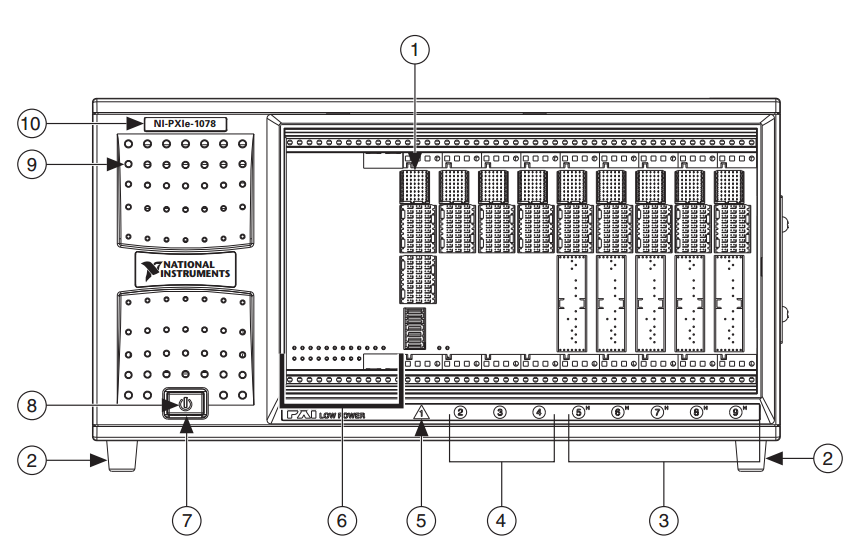
\includegraphics[scale=0.4]{FiguresP/pxi}
%\caption{NI PXIe-1078}
%\label{fig:pxi}
%\end{figure}


\begin{figure}[htb!]
\centering
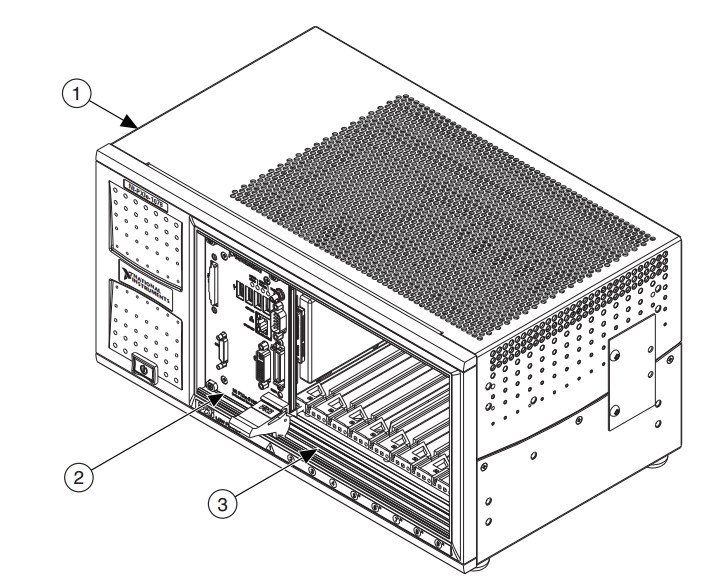
\includegraphics[scale=0.4]{FiguresP/pxi2}
\caption{NI PXIe-1078 con su controlador embebido}
\label{fig:pxi_ebedded_controller}
\end{figure}



El sistema NI PXIe-1078 con el que se está trabajando tiene las siguientes especificaciones:
\begin{itemize}
\item 5 ranuras híbridas, 3 ranuras PXI Express
\item 300 W de potencia total disponible desde 0 a 50 ºC
\item Rendimiento medio - Ancho de banda hasta250 MB/s por ranura y ancho de banda del sistema de 1 GB/s
\item Chasis de poca profundidad de 8.43 in. (214.2 mm) 
\item Compatibilidad con módulos PXI, PXI Express, CompactPCI y CompactPCI Express
\end{itemize}






%The NI PXIe-1078 chassis kits consist of a low-cost, 9-slot chassis featuring a 4-slot-wide system controller slot, which can accept either an embedded controller or remote controller, and eight peripheral slots. The NI PXIe-1078 offers the flexibility to populate each peripheral slot with a PXI Express module or populate up to five slots with PXI modules. In addition, it features compact, rugged packaging, and quiet operation, which make it ideal for portable, desktop, and industrial control applications






\subsection*{Módulo de adquisición de datos NI PXIe-6363 (figura \ref{fig:daq})}

\begin{itemize}
\item 32 entradas analógicas, 2 MS/s monocanal, 1.25 MS/s multicanal, resolución de 16 bits, $\pm$ 10 V
\item Cuatro salidas analógicas, 2.86 MS/s, resolución de16 bits, $\pm$ 10 V
\item 48 líneas de E/S digital (32 temporizadas por hardware hasta 10 MHz)
\item Cuatro contadores/temporizadores de 32 bits para PWM, codificador, contar eventos y más
\item Disparo analógico y digital y temporización 
\item Soporte para Windows 7/Vista/XP/2000
\end{itemize}



\begin{figure}[htb!]
\centering
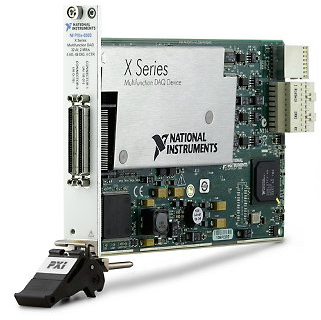
\includegraphics[scale=0.5]{FiguresP/pxi6363}
\caption{Módulo de adquisición de datos NI PXIe-6363}
\label{fig:daq}
\end{figure}


Para conectar los modulos de adquisicion de datos con las señales provenientes de los sensores se usa un m\'odulo de conexiones como el que se muestra en la figura \ref{fig:conexionPXI}.



\begin{figure}[htb!]
\centering
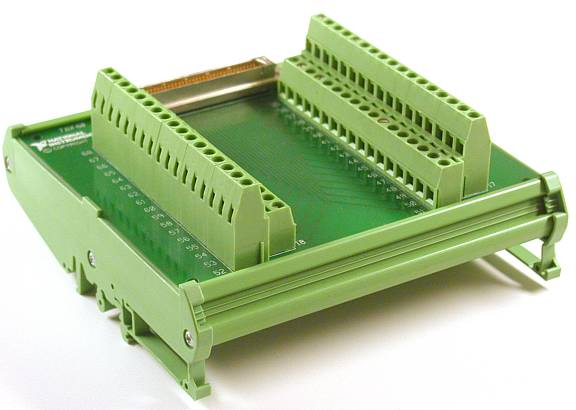
\includegraphics[scale=0.15]{FiguresP/NI-TBX-68}
\caption{Conector exterior para modulos de adquisicion PXI}
\label{fig:conexionPXI}
\end{figure}


En la tabla \ref{tab:signalsMaster} se muestra un listado de las señales digitales y analógicas del dispositivo maestro.

\newpage
\begin{sidewaystable}[htbp]
  \centering
  \caption{Listado de señales del robot maestro}
    \begin{tabular}{lllccccc}
    \toprule
    \multicolumn{8}{c}{\textbf{LISTADO DE SEÑALES ROBOT MAESTRO}} \\
    \hline
    \multicolumn{1}{c}{\multirow{2}{*}{\textbf{TAG}}} & \multicolumn{1}{c}{\multirow{2}{*}{\textbf{ORIGEN}}} & \multicolumn{1}{c}{\multirow{2}{*}{\textbf{DESCRIPCIÓN}}} & \multicolumn{1}{c}{\multirow{2}{*}{\textbf{TIPO SEÑAL}}} & \multicolumn{4}{c}{\textbf{SEÑAL}} \\  
  &  &  & & \textbf{DI} & \textbf{DO} & \textbf{AI} & \textbf{AO} \\
    \hline
   MAS-MSA & Maestro, Motor SA & Ref Motor, Salida Analógica, $\pm$10V & Comando &       &       &       & 1 \\
    MAS-MSE & Maestro, Motor SE & Ref Motor, Salida Analógica, $\pm$10V & Comando &       &       &       & 1 \\
    MAS-MEL & Maestro, Motor EL & Ref Motor, Salida Analógica, $\pm$10V & Comando &       &       &       & 1 \\
    MAS-MWY & Maestro, Motor WY & Ref Motor, Salida Analógica, $\pm$10V & Comando &       &       &       & 1 \\
    MAS-MWP & Maestro, Motor WP & Ref Motor, Salida Analógica, $\pm$10V & Comando &       &       &       & 1 \\
    MAS-RSA & Maestro, Motor SA & Ref Motor, Salida Analógica, $\pm$10V & Comando &       &       &       & 1 \\
    MAS-RSE & Maestro, Motor SE & Ref Motor, Salida Analógica, $\pm$10V & Comando &       &       &       & 1 \\
    MAS-REL & Maestro, Motor EL & Ref Motor, Salida Analógica, $\pm$10V & Comando &       &       &       & 1 \\
    MAS-RWY & Maestro, Motor WY & Ref Motor, Salida Analógica, $\pm$10V & Comando &       &       &       & 1 \\
    MAS-RWP & Maestro, Motor WP & Ref Motor, Salida Analógica, $\pm$10V & Comando &       &       &       & 1 \\
    MAS-PSA & Maestro, Potenciómetro SA & Potenciómetro Alimentado $\pm$10V & Medida &       &       & 1     &  \\
    MAS-PSE & Maestro, Potenciómetro SE & Potenciómetro Alimentado $\pm$10V & Medida &       &       & 1     &  \\
    MAS-PEL & Maestro, Potenciómetro EL & Potenciómetro Alimentado $\pm$10V & Medida &       &       & 1     &  \\
    MAS-PWY & Maestro, Potenciómetro WY & Potenciómetro Alimentado $\pm$10V & Medida &       &       & 1     &  \\
    MAS-PWP & Maestro, Potenciómetro WP & Potenciómetro Alimentado $\pm$10V & Medida &       &       & 1     &  \\
    MAS-PWR1 & Maestro, Potenciómetro WR1 & Potenciómetro Alimentado $\pm$10V & Medida &       &       & 1     &  \\
    MAS-PWR2 & Maestro, Potenciómetro WR2 & Potenciómetro Alimentado $\pm$10V & Medida &       &       & 1     &  \\
    MAS-PGRP & Maestro, Potenciómetro Gripper & Potenciómetro Alimentado $\pm$10V & Medida &       &       & 1     &  \\
    MAS-SHALT & Maestro, Pulsador Halt / Resume & Pulsador Sostenido & Pulsador & 1     &       &       &  \\
    MAS-SHYD & Maestro, Pulsador Hidráulica & Pulsador & Pulsador & 1     &       &       &  \\
    MAS-SWR & Maestro, Pulsador Wrist Mode & Pulsador & Pulsador & 1     &       &       &  \\
    MAS-SGRP & Maestro, Pulsador Gripper Lock & Pulsador & Pulsador & 1     &       &       &  \\
    MAS-LGRP & Maestro, Led Gripper Lock & Indicación, Led 5V, 15mA & Led   &       & 1     &       &  \\
    MAS-LWR & Maestro, Led Wrist Mode & Indicación, Led 5V, 15mA & Led   &       & 1     &       &  \\
    MAS-LHALT & Maestro, Led Halt / Resume & Indicación, Led 5V, 15mA & Led   &       & 1     &       &  \\
    MAS-LHYD & Maestro, Led Hidráulica & Indicación, Led 5V, 15mA & Led   &       & 1     &       &  \\
    \hline
    \multicolumn{4}{r}{\textbf{TOTAL}} & 4 & 4 & 8 & 10 \\
    \hline
    \end{tabular}%
  \label{tab:signalsMaster}%
\end{sidewaystable}%



